%%%%%%%%%%%%%%%%%%%%%%%%%%%%%%%%%%%%%%%%%
% Simple Sectioned Essay Template
% LaTeX Template
%
% This template has been downloaded from:
% http://www.latextemplates.com
%
% Note:
% The \lipsum[#] commands throughout this template generate dummy text
% to fill the template out. These commands should all be removed when 
% writing essay content.
%
%%%%%%%%%%%%%%%%%%%%%%%%%%%%%%%%%%%%%%%%%

%----------------------------------------------------------------------------------------
%	PACKAGES AND OTHER DOCUMENT CONFIGURATIONS
%----------------------------------------------------------------------------------------

\documentclass[12pt]{article} % Default font size is 12pt, it can be changed here

\usepackage{listings}
\lstset{
    basicstyle=\ttfamily,
    mathescape
}

\usepackage{hyperref}

% \usepackage{geometry} % Required to change the page size to A4
% \geometry{a4paper} % Set the page size to be A4 as opposed to the default US Letter

\usepackage{graphicx} % Required for including pictures
\graphicspath{ {img/} }
\usepackage{amsfonts}
\usepackage{amsmath}

\usepackage{float} % Allows putting an [H] in \begin{figure} to specify the exact location of the figure
\usepackage{wrapfig} % Allows in-line images such as the example fish picture

\usepackage{lipsum} % Used for inserting dummy 'Lorem ipsum' text into the template

\linespread{1.0} % Line spacing

%\setlength\parindent{0pt} % Uncomment to remove all indentation from paragraphs

%\graphicspath{{Pictures/}} % Specifies the directory where pictures are stored

\begin{document}

\title{Independent Study Report}
\author{Wei Zhong}
\date{}

\maketitle

\section{Abstract}
This report summarizes the work on building query autocompletion system for math retrieval, it gives a survey on previous related research on autocompletion, including traditional text query auto completion and systems based on graph database. A prototype system has been built to demonstrate the usability of such system. We also evaluate the query autocompletion system effectiveness through some case analysis.

\section{Introduction}
In information retrieval, query auto completion (QAC), also known as type-ahead and auto-complete suggestion, is the functionality to help user suggest the complete query when user only inputs a number of characters of incomplete query.
The user interface returns a set of candidate queries 
to guess user's intent or suggest better queries.
This functionality can reduce user keystrokes and improve user experience.
The cuts down on search duration of users also implies a lower load on the search engine.

On the other hand, math search is a crucial aspects of information retrieval, because of the presence of scientific digital asset and its great value to society and innovation, many formula search engines have been proposed and studied in recent efforts.
Also, academic search and math retrieval has been shown to be useful in scientific knowledge mining and retrieval.
However, although several math search engine has been available to public, the QAC facility offered in traditional text search engines are not yet become accessible to users.
Furthermore, math expression is difficult to input because the heavy structured characteristic and 
usually the commonly used TeX format involves a lot of typing compared to traditional text oriented search engine QAC system.
Also, the data that math search engine indexes are domain-specific corpus and currently not too many relevance judgements are conducted on math QAC system.
We here propose a QAC system for math equation,
with interactive query completion interface and a suggestion model designed for math formula that does not only address prefix matching but also consider matching from the middle and structure commutativity. Because traditional prefix based QAC system only recommends queries for prefixes that have been previously seen by the search engine.
To address the issue of absence of math QAC query log and the information on actual user interaction.
This paper also reviews the literature on QAC and provides a general understanding of QAC approaches that are currently available.
We try to use the corpus to model frequency.
The main contribution of the current work is that we show the potential value of query
term suggestion in math search.

\section{Related Work}
\subsection{Text query auto completion}
\cite{cai_survey_2016}
\cite{di_santo_comparing_2015}
give a good summary on different auto-completion methods and their relevance
performance.
\cite{di_santo_comparing_2015} focuses on ranking approaches for query suggestion.
Methods can be divided into popularity-based, time-based and similarity-based.
Popularity-based methods use the frequency of query candidates past popularity (MPC as referred by Bar-Yossef), or the document frequency of candidate query (Sentence occurrence) in the literature or
query log. Term occurrence ranker (TO) introduces TF-IDF and combine it with term popularity.
Time-based approaches base on session information, in time ranker (TR), ranker scores by the time elapsed from the most recent past occurrence in query log. Most-popular time ranker (MT) combines popularity with MT.
Lastly, similarity-based methods weight query candidate by their similarity to user query log or the documents user previously clicked. The similarity can be measured by proximity (e.g. Near words), string similarity, or context similarity (e.g. N-Gram similarity, semantic similarity).
For example, \cite{schmidt_context_sensitive_2016} uses entity to restrict suggestion results in a given category specified by user. 
And in \cite{mitra_exploring_2015}, Convolutional Latent Semantic Model is applied for query reformulations similarity by offset of vector.
They train the data based on succession query pair in user session in addition to clickthrough data,
to infer more contextually relevant query suggestions.
They found context similarity is good at understanding the actual user intent when only a few characters have been entered in which case MPC will perform poorly.
Reportedly, models trained on session pairs perform better than those trained on clickthrough data, and supervised learning-to-rank models perform better than
those trained with similarity features alone.
Search context can also be used to personalize query auto completion, this involves aggregating list of query logs in order to compare their hybrid similarity to search context.

Survey \cite{cai_survey_2016} names alternative two broad categories: Heuristic models and learning based models, depending on applying machine learning method or not.
The heuristic models are further divided into time-sensitive (e.g. MPC variances), and user-centered (e.g. personalization using session context~\cite{schmidt_context_sensitive_2016}).
For example, user's implicit negative feedback such as skipped query completion, eye contact can also be used as feedback.
Learning based models have adopted many features to evaluate suggestions, Likelihood ratio (LLR) and query relatedness are used in \cite{chien_semantic_2005} which captures a pair of query correlation based on their popularity behavior over time. Other learning features include user log features~\cite{kharitonov_user_2013}, query entity discover~\cite{guo_named_2009}, demographic-based features~\cite{shokouhi_learning_2013}, etc.
\cite{kharitonov_user_2013} learns model from query log of Yandex,
it defines a query-term graph to model likelihood of a sequence of query prefix. Their
method is basically searching in the graph the continuing paths with product of
the probabilities of their edges are among the N highest, the procedure is able to
prune candidate whose maximum probability is lower than the current candidate
by depth-first search.
The survey also relates the subtle differences between query suggestion, query expansion and query correction.

\subsection{Evaluations}
Cai et al. \cite{cai_survey_2016} covers evaluation for query auto completion extensively.
It identifies three major query logs (AOL, MSN and SogouQ) used in query autocompletion training/evaluation.
As for evaluation metrics, 
it is acknowledged in \cite{bhatia_query_2011} that precision is much more important metric than recall as the number of suggestions can be offered is often very limited in space.
Transitional retrieval evaluation metrics, such as MAP (Mean Average Precision), success rate at top-K (SR@K) and nDCG/$\alpha-$nDCG are also used to assess suggestion quality for diversified query autocompletion systems~\cite{cai_survey_2016}.
Among these metrics, according to the survey, MRR is used widely as ``standard measurement'' where the rank of final query submitted by user (target query) is used to value query suggestions.
Various forms of reciprocal rank are used, for example, \cite{bar-yossef_context-sensitive_2011} uses session log, the quality of suggestion is determined by reciprocal rank
of the user query, weighted by the number of completions given for a prefix. This addresses the different difficulty from completing different prefix (e.g. "prefix starting from z versus starting from c").
\cite{kharitonov_user_2013} tries to propose a specific evaluation model for query autocompletion, it combines a user behaviour graph model and their key presses effort, their metrics can reflect user behaviour better on long queries.
query clarity score  \cite{bhatia_query_2011, predicting_2002}, it increases as adding more specific terms that reduce query ambiguity.

The other direction is assessing the efforts saved to help user complete target query. 
MKS (Minimal Keystrokes) by \cite{duan_online_2011}
is used in query suggestion system evaluations~\cite{kharitonov_user_2013}, although it is initially proposed to evaluate the query misspelling correction algorithm.



\subsection{Text QAC Problems}
Unseen prefixes is one common issue in text query auto completion.
In typical query auto-completion systems, candidate query are generated from prefix lookup against candidate query set (e.g. query log), however, these systems
 can only recommend queries for prefixes that have been previously seen by the search engine with adequate frequency.
\cite{mitra_query_2015} explores the idea to use suffixes that are popular n-grams and append it to current query prefix.
Their experiment shows, compared to baseline setting in, their model is as good as MPC for previously seen queries and outperform MPC by 43\% in MRR for previously unseen queries.
\cite{park_neural_2017} proposes a language model that employs  recurrent neural network to resolve the dimensionality problem with a distributed representation of text.
It shows this can boost the query suggestion for both seen and unseen prefixes.
This study, unlike term-level query auto completion in \cite{vargas_term-by-term_2016}, can handle Out-of-Vocabulary words because of character-level query completion.
On the other hand, for many popularity based methods, the models assume the current query popularity distribution will remain the same as that previously observed but this is not suitable for time-sensitive changes such as breaking news topic. This is addressed by only take a window size of past query log evidence to improve temporal sensitivity of popularity based methods~\cite{cai_survey_2016}.
Another approach to address time temporal issue is using time-series analysis, and put emphasis on ``trending'' keywords~\cite{shokouhi_detecting_2011}.
Research in this direction tries to detect ``bursts'' in query frequencies of recent query log.

\subsection{Math formula autocompletion}
Math formula autocompletion is a new research domain, to my best knowledge, there is no paper published in this particular area. 
Popular math search system WolframAlpha supports math expression autocompletion, although their system is closed, we can observe the query candidates is filtered by matching string prefix of math expressions. 
Thus, math expressions with commutative operator or using a different set of symbols will not show up as suggestions.
We argue that math formula autocompletion should be aware of the unique characters of math expression such as community, associativity, sub-expression similarity (one expression is relevant to the other by being a subexpression, and a subexpression can match any place in the middle, not necessarily match the prefix) and symbol set unification (symbols can be used interchangeably across similar math expressions).
Given these, the uniqueness of math expression remains to be defined in the query autocompletion context, since math expressions with same meaning may have different string representations. Otherwise the MPC method used in normal text completion cannot simply be applied in math query autocompletion.

Dealing with math formula autocompletion may need to use existing math formula search engines or utilize some graph-based database (such as Neo4j) to identify the unique math expressions/subexpressions and retrieve similar math expressions by subexpressions (rather than using string prefix/suffix).

\section{Methodology and implementation}
Most popular completion (MPC) is most commonly used metrics to generate query completion from query
log.
MPC is a method that prioritizes query autocompletion suggestions based on the candidate frequency in history (e.g. query log).
MPC has been used as baseline for evaluation in many QAC systems.
Since math QAC system is a new research topic, a good starting point is to base on math formula frequency to rank suggested queries.
Here we describe the algorithm and implementation of query autocompletion based on frequency of math formula.

Since math expressions can use different symbol set but have the same semantic meaning, also, the operands can have different order in commutative operators,
in many math search engines usually structure-similar expressions are filtered out first rather than those only matching the symbols.
And if symbol set matches better, it is prioritized.
On the other hand, text query completion usually filter candidate queries by their string prefix or suffix, thus the traditional filtering of QAC completion candidates are not meeting the demand of math search QAC scenario.

To generate query completion from MPC based metrics, we first define the uniqueness of math expression by a similarity threshold.
Two math expressions are unique if they are not identical.
Let $t$ be a math expression, the set of expressions that are identical to this math expression is defined by $U(t)$ in which all the math expressions have the similarity level higher to a threshold value $\theta$:
$$
U(t) = \{s: \text{sim}(s, t) \ge \theta\}
$$
this way we not only utilize current math expression similarity metrics,
but also increase tolerance on what is called an identical math expression to allow operand reordering and using different symbol set.
The similarity measurement function $\text{sim(s,t)}$ takes both structure similarity and symbol set similarity into account.
Structure similarity is helpful because we do not want a simple query will give us a very complex and large expression, and symbol set similarity is also helpful because we do want to differentiate the expressions such as $ax^2$ and $mc^2$.
On the other hand, we also want to save user keystrokes, this requirement from QAC needs the combination of estimated probability on user target query (e.g. frequency in query log) and the similarity of query and target query.

Give the definition of uniqueness, we assign identical math expressions a same expression ID (exprID). They are indexed in math search engine index just as if they are indexed for similarity search except the following differences:
\begin{itemize}
\item Identical expressions are only indexed once
\item Each time an identical expression input will increase its frequency, the frequency is further
indexed
\end{itemize}

In our exploratory system, the threshold $\theta$ is fixed to 0.9,
thus if any indexed expression has a similarity score larger than
the threshold, it is treated as identical expressions, and the frequency will
increase onto the expression ID which represents the unique expressions.
Otherwise, it is an unique expression, and will be indexed with a separate
expression ID with an initial frequency equals to one.
Although we have utilized the existing similarity search, the
downside of measuring uniqueness by a thorough search per indexing
expression is that it largely increases index time.

At query time, we again use similarity measurement function $\text{sim(s,t)}$ 
to rank suggestions.
We have tried using similarity only (without considering frequency) ranking function $R_1 = \text{sim(s,t)}$, however, the suggested formula is very monotonic in length.

Below is an example of only ranking completions by their similarity to incomplete query:
\begin{center}
\begin{tabular}{lr}
Top completions $\backslash$ Query  & $ ax + $ \\
\hline
 1 &  $ ax^2 + bx $ \\
 2 &  $ πr^2 + E(r) $\\
 3 &  $ xy + yx^2$ 
\end{tabular}
\end{center}

This indicates we may further include the frequency $f_t$ of
each query expression candidate $t$ as factor to rank math QAC results.
The intuition is to bridge the balance between the target query which often
is more complex and longer formula,
with the completion candidate similarity (e.g. the input expression being subexpression of completion candidates).

To include frequency, we have tried using scoring function below to rank candidate completions
$$
\text{score} = \frac{s \cdot f}{\log(1 + l)}
$$
where s is scaled similarity score produced by math search engine similarity
measurement (including structural and symbolic similarity), l is search level
which represents the differences in size and depth of subexpression relation.
And f is the frequency of that unique expression.
The basic idea for this scoring formula is that we want to penalize 
large completion candidate but this penalty should not be too much.
Since a large but good suggestion (e.g. popular) can save user more
keystrokes.

We have also tried to apply symbol sequence similarity to our completion candidates' ranking.
Symbol sequence is the sequence of operand symbols in the tree leaves, even they are under
commutative operands. Our initial thought is trying to use this information to distinguish
expressions like $a + b$ and $b + a$ which only differs in the symbol sequence.
We applied longest common substring algorithm to measure this similarity.
However, it turns out not only the query processing time is more than doubled, but also 
few case in all examples that we found it would help quality of completion.
Because the results are not good, they are not shown in this report and the symbol sequence idea
is left for further exploration.

\subsection{System implementation}
To demonstrate math QAC system usability, a system prototype is built.
Auto completion facility is mainly WEB UI and it is based on previous Approach0 system.
Currently the query processing is sending query to Approach0 backend and get
query auto completion results back, these results are returned by the QAC search daemon module
using model previously stated.
The Web frontend is composed by Vue component.
We created a Nodejs daemon relay the request from frontend to URI hosted by QAC search daemon module. 
\begin{figure}
\begin{center}
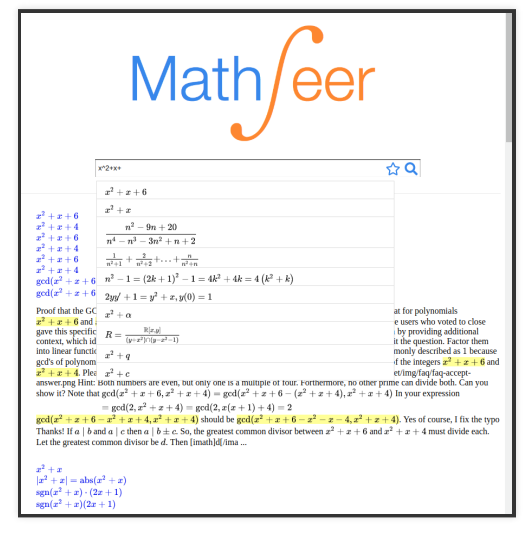
\includegraphics[height=6cm]{qac-system-suggest}
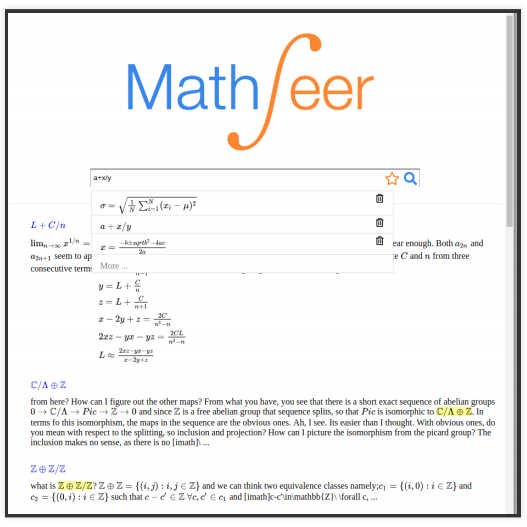
\includegraphics[height=6cm]{qac-system-star}
\caption{Math QAC interface. From left to right: the QAC suggestion list and stared list for saving frequently searched formula}
\end{center}
\end{figure}

The system process can be divided into two stages.

In index stage, document math expressions are
indexed in such a way that only an “unseen" (by the definition of our uniqueness) expression is
indexed, and its frequency in query log is initially set to one (frequency value is stored in a key-value database where its value is mapped to an expression ID).
Later
if the same expression is appended into query log, we will first parse the TeX expression of query, identify this expression has been previously indexed by going to its corresponding corresponding index node and find if there is any expression has a certain level of similarity (within a threshold score) with the query. If that is the case, the document expression ID is obtained.
Then we update the frequency in the key-value database.

In search stage, if a query is entered, we search for the math expression index and find any expressions
matches either match exactly to the query or having the query expression being a sub-expression, if any
such document expression is found, we retrieval the expression as well as the frequency value it
associates (from key-value database) and rank the suggested expressions by their frequency and other similarity factors given by a scoring formula.
%
The algorithm pseudo code below concludes the general index and search process:
\vspace{0.5cm}
\begin{lstlisting}
Function index(tex)
    result := math_expr_search(tex);
    if result is not empty:
        for r in result:
            if r.score > threshold:
                key_value_db[r.exprID].freq += 1
    else:
        operator_tree := parse(tex)
        if no parser error reported:
            cur_len := len(key_value_db)
            new_exprID := cur_len + 1
            key_value_db[new_exprID].freq := 1
            Index math expression by operator_tree

Function search(tex)
    result := math_expr_search(tex);
    for each result f := key_value_db[new_exprID].freq
    rank result by scoring formula
\end{lstlisting}

\section{Results and Discussion}
We have evaluated the proposed method using Wikipedia dataset published in NTCIR-12.
There are 591,468 formula in Wikipedia corpus from NTCIR-12 Formula Browser
task, 132,372 structrually unique TeX expressions (using our defined uniqueness) obtained
after indexing.

We report some selected query autocompletion examples that have been evaluated under our system.
Each query input process is divided into several tables to show the intermediate suggestions
from each input state (assume the user input cursor is at the end of query).
Our QAC backend generates the returned completion results with their frequency information and
ranking score.

\subsection{Query $x^2+y$}
\begin{center}
\begin{tabular}{lccc}
Suggesions $\backslash$ Query  & $x^2 $ & Frequency & Score \\
\hline
 1 &  $ O(R^{2})\,\! $ & 302 & 46.85 \\
 2 &  $ r^{2}m $ & 165 & 32.26 \\
 3 &  $ q\sim p^{2} $ & 131 & 25.61 \\
 4 &  $ f^{2}(\theta) $ & 84 & 16.42 \\
\end{tabular}
\end{center}

\begin{center}
\begin{tabular}{lccc}
Suggesions $\backslash$ Query  & $x^2+ $ & Frequency & Score \\
\hline
 1 &  $ x^{2}+y^{2}=r^{2}.\! $ & 100 & 9.80 \\
 2 &  $ \scriptstyle r=\sqrt{a^{2}+b^{2}} $ & 44 & 3.63 \\
 3 &  $ x^{2}+y^{2}=1 $ & 25 & 2.95 \\
 4 &  $ \sqrt{a^{2}+b^{2}} $ & 19 & 2.37 \\
\end{tabular}
\end{center}


\begin{center}
\begin{tabular}{lccc}
Suggesions $\backslash$ Query  & $x^2 + y$ & Frequency & Score \\
\hline
 1 &  $ f(x)=x^{3}+x $ & 11 & 1.61 \\
 2 &  $ x^{2}+px+q=0 $ & 12 & 1.41 \\
 3 &  $ f_{c}(z)=z^{2}+c $ & 9 & 1.05 \\
 4 &  $ z\mapsto\bar{z}^{2}+c\,. $ & 5 & 0.98 \\
\end{tabular}
\end{center}

%%%%%%%%%%%%%%%%%%%%%%%%
%%%%%%%%%%%%%%%%%%%%%%%%
%%%%%%%%%%%%%%%%%%%%%%%%
%%%%%%%%%%%%%%%%%%%%%%%%

\subsection{Query $ax^2+b$}

\begin{center}
\begin{tabular}{lccc}
Suggesions $\backslash$ Query  & $ ax $ & Frequency & Score \\
\hline
 1 &  $ d_{BO}\!\,- $ & 2667 & 412.08 \\
 2 &  $ \mathbf{F}=m\mathbf{g} $ & 1287 & 250.84 \\
 3 &  $ x_{\mathrm{new}} $ & 829 & 102.68 \\
 4 &  $ b^{th} $ & 521 & 80.50 \\
\end{tabular}
\end{center}

\begin{center}
\begin{tabular}{lccc}
Suggesions $\backslash$ Query  & $ ax^2 $ & Frequency & Score \\
\hline
 1 &  $ I=r^{2}m $ & 96 & 18.77 \\
 2 &  $ O(VE^{2}) $ & 38 & 5.90 \\
 3 &  $ q\,=\,\tfrac{1}{2}\,\rho\,v^{2} $ & 47 & 5.50 \\
 4 &  $ P=wc^{2}\rho $ & 34 & 4.98 \\
\end{tabular}
\end{center}

\begin{center}
\begin{tabular}{lccc}
Suggesions $\backslash$ Query  & $ ax^2 + $ & Frequency & Score \\
\hline
 1 &  $ ax^{2}+bx+c=0 $ & 19 & 1.86 \\
 2 &  $ y=ax^{2}+bx+c\, $ & 38 & 1.57 \\
 3 &  $ \ p(x)=ax^{2}+bx+c $ & 14 & 1.17 \\
 4 &  $ ax^{2}+bx=c $ & 6 & 0.71 \\
\end{tabular}
\end{center}

\begin{center}
\begin{tabular}{lccc}
Suggesions $\backslash$ Query  & $ ax^2 + b $ & Frequency & Score \\
\hline
 1 &  $ ax^{2}+bx+c=0 $ & 19 & 2.23 \\
 2 &  $ y=ax^{2}+bx+c $ & 16 & 1.88 \\
 3 &  $ \ p(x)=ax^{2}+bx+c $ & 14 & 1.37 \\
 4 &  $ a+b\alpha+c\alpha^{2}, $ & 5 & 0.62 \\
 5 &  $ \sqrt{a+bz+cz^{2}} $ & 4 & 0.52 \\
\end{tabular}
\end{center}

%%%%%%%%%%%%%%%%%%%%%%%%
%%%%%%%%%%%%%%%%%%%%%%%%
%%%%%%%%%%%%%%%%%%%%%%%%
%%%%%%%%%%%%%%%%%%%%%%%%

\subsection{Query $(1+ \frac 1 n)^n$}

\begin{center}
\begin{tabular}{lccc}
Suggesions $\backslash$ Query  & $ 1+ $ & Frequency & Score \\
\hline
 1 &  $ \displaystyle a_{n+1} $ & 319 & 39.91 \\
 2 &  $ (y+1) $ & 95 & 18.68 \\
 3 &  $ N=M+1\, $ & 59 & 8.71 \\
 4 &  $ m=+1 $ & 44 & 8.65 \\
 5 &  $ F(n+1) $ & 51 & 6.38 \\
\end{tabular}
\end{center}

\begin{center}
\begin{tabular}{lccc}
Suggesions $\backslash$ Query  & $ 1+\frac 1 n $ & Frequency & Score \\
\hline
 1 &  $ 1+\frac{1}{\varphi}=\varphi $ & 4 & 0.78 \\
 2 &  $ \frac{1}{r}+\frac{1}{p}=1+\frac{1}{s} $ & 3 & 0.29 \\
 3 &  $ e=\lim_{n\to\infty}\left(1+\frac{1}{n}\right)^{n}. $ & 6 & 0.27 \\
 5 &  $ \frac{n+1}{n}=1+\frac{1}{n} $ & 2 & 0.24 \\
\end{tabular}
\end{center}

\begin{center}
\begin{tabular}{lccc}
Suggesions $\backslash$ Query  & $ (1+\frac 1 n) $ & Frequency & Score \\
\hline
 1 &  $ e=\lim_{n\to\infty}\left(1+\frac{1}{n}\right)^{n}. $ & 6 & 0.32 \\
 2 &  $ (1+1/n)^{n} $ & 2 & 0.31 \\
 3 &  $  \lim_{n\to\infty}\left(1+\frac{1}{n}\right)^{n} $ & 4 & 0.29 \\
 4 &  $ P(1+1/{\epsilon})=MC $ & 2 & 0.21 \\
 5 &  $ (1+1/n)r $ & 1 & 0.20 \\
\end{tabular}
\end{center}

\begin{center}
\begin{tabular}{lccc}
Suggesions $\backslash$ Query  & $ (1+\frac 1 n)^n $ & Frequency & Score \\
\hline
 1 &  $ e=\lim_{n\to\infty}\left(1+\frac{1}{n}\right)^{n}. $ & 6 & 0.53 \\
 2 &  $  \lim_{n\to\infty}\left(1+\frac{1}{n}\right)^{n} $ & 4 & 0.47 \\
 3 &  $ \lim_{x\to+\infty}\left(1+\frac{1}{x}\right)^{x}=e $ & 1 & 0.09 \\
 4 &  $ \lim_{n\to\infty}\left(1+\frac{1}{n}\right)^{n}, $ & 1 & 0.08 \\
 5 &  $ \left(1+\frac{1}{x}\right)^{x}<e<\left(1+\frac{1}{x}\right)^{x+1} $ & 1 & 0.07 \\
\end{tabular}
\end{center}

As we can see from these results, when query is getting more complete, the results are obviously
getting better, however, at the very first input state, e.g. $x^2$ and $ax$ in query 5.1 and query 5.2, they are actually getting very counter intuitive results.
We assume the main reason is small formula (such as $r^2m$) has a large frequency that dominates the
first generated results when inputting query is also small, and the symbol set similarity is overshadowed in this case, thus visually it is very far from good autocompletion results at that stage.
For relative more complete input queries, the completion results are more constrained and looks more accurate even we do not know the target query.

From these results we can know that it might be worth investing for future research that,
either use different model for different stage of input or come up a better scoring formula that
penalize more on symbol set similarity when input query is far from complete.
It is also important to try to speedup the identification of uniqueness and test if an existing unification equivalent expression has been already indexed. Since the current index method needs to perform a similarity search on existing index which is very costly if it is performed for every indexing formula.

\section{Conclusion}
In this report, we have done some explorations on applying the idea of query autocompletion in
typical text search engine to math formula search engine.
Specifically, we rank the generated relevant formula by a classical schema: Most popular completion (MPC).
Due to the characteristics of math formula, we have to identify the uniqueness of math formula with the consideration of symbol unification, symbol set similarity, symbol sequence similarity and structure similarity (subexpression and operand commutativity).
We propose a uniqueness definition based on a overall similarity filter (controlled by a threshold value) and apply a scoring formula that take addressed factors into consideration. 
Results show the symbol sequence similarity will make little difference on completion results and it
also conflicts with unified index since unified expressions are only indexed once.
The results of almost complete query are intuitively better, but the early input stage when query are
far from complete are not looking very relevant. Future work may address this problem by emphasising the symbol similarity when query input is just begin.
\bibliography{main}{}
\bibliographystyle{plain}
\end{document}
